\documentclass[11pt,a4paper]{article}
\usepackage{algorithmicx}
\usepackage{algpseudocode}
\usepackage[ruled,vlined,linesnumbered,algosection,algo2e]{algorithm2e}
\newtheorem{theorem}{Theorem}[section]
\newtheorem{algorithm}[theorem]{Algorithm}
\usepackage{amsmath, amsfonts, amssymb}
\usepackage{graphicx}
\usepackage[left=2.00cm, right=2.00cm, top=2.00cm, bottom=2.0cm]{geometry}
\usepackage[english]{babel}
\usepackage[utf8]{inputenc}
\usepackage{fancyhdr}
\usepackage{titlesec}
\usepackage{amsmath}
\usepackage{multirow}
\usepackage{float}
\usepackage{hyperref}

\titlelabel{\thetitle.\quad}

\pagestyle{fancy}
\fancyhf{}
\rhead{Data Structures and Algorithms}
\lhead{Lab 3: Sorting}
\rfoot{Page \thepage}

\newcommand\tab[1][1cm]{\hspace*{#1}}
\newcommand{\horrule}[1]{\rule{\linewidth}{#1}}
\title{
\normalfont \LARGE
\textsc{University of Science} \\ [25pt] % Your university, school and/or department name(s)
\horrule{1pt} \\[0.4cm] % Thin top horizontal rule
\huge Sorting Algorithms - An Overview \\ % The assignment title
\horrule{1pt} \\[0.6cm] % Thick bottom horizontal rule adjust 0.6cm suitably
\Large Data Structures and Algorithms\\[0.5cm]  %% sub title, adjust \Large
}

\author{Huynh Minh Tuan - 20120024@student.hcmus.edu.vn}
\date{November 2021}

\begin{document}

\maketitle

\begin{abstract}
    Sorting is nothing but alphabetizing, categorizing, arranging, or putting items in an ordered sequence. 
    It is a key fundamental operation in the field of computer science. It is of extreme importance because it adds usefulness to data.
    In this report, I have compared eleven common sorting algorithms (Selection Sort, Insertion Sort, Bubble Sort, Shaker Sort, Shell Sort, Heap
    Sort, Merge Sort, Quick Sort, Counting Sort, Radix Sort, and Flash Sort). I have developed a program in C++, Python and experimented with several input sizes
    10,000, 30,000, 50,000, 100,000, 300,000, and 500,000 elements. The performance and efficiency of these algorithms in terms of CPU time consumption 
    as well as the number of comparisons that have been recorded and presented in tabular and graphical form.
\end{abstract}

\section{Introduction}
\tab Sorting is not a leap but it has emerged in parallel with the development of the human mind.
In computer science, alphabetizing, arranging, categorizing, or putting data items in an ordered sequence on the basis of similar properties is called sorting.
Sorting is of key importance because it optimizes the usefulness of data.
We can observe plenty of sorting examples in our daily life, e.g. we can easily find required items in a shopping mall or utility store because the items are kept categorically.
\newline
\newline
\tab The items to be sorted may be in various forms i.e. random as a whole, already sorted, very small or extremely large in numer, sorted in reverse order etc.
There is no algorithm that is best for sorting all types of data. 
We must be familiar with sorting algorithms in terms of their suitability in a particular situation.
\newline
\newline
\tab In this paper, I am going to compare eleven common sorting algorithms (Selection Sort, Insertion Sort, Bubble Sort, Shaker Sort, Shell Sort, Heap
Sort, Merge Sort, Quick Sort, Counting Sort, Radix Sort, and Flash Sort) for their CPU time consumption and number of compared operations on four different data arrangements 
(Sorted data (in ascending order), Nearly sorted data, Revherse sorted data, and Randomized data).


\section{Algorithm presentation}
\subsection{Selection Sort}

\subsubsection*{Idea}
The Selection Sort is based on the idea of finding the minimum element in an unsorted array and then putting it in its correct position in a sorted array.

\subsubsection*{Pseudo code}
\begin{algorithm2e}
  \KwIn{$a_1, a_2, ..., a_N$}
  \KwOut{$a_1, a_2, ..., a_N$ (in sorted)}
  \SetAlgoLined
  \For{$i \gets 1$ to $N$}{
    $minIndex \gets i$\\
    \For{$j \gets i+1$ to $N$}{
        \If{$a_{minIndex} > a_{j}$}{
            $minIndex \gets j$
        }
    }
    swap($a_{minIndex}$, $a_{i}$)
  }
  \caption{Selection Sort}
\end{algorithm2e}

\subsubsection*{Complexity}
Best case time complexity: $O(N^2)$ \\
Worst case time complexity: $O(N^2)$ \\
Worst case space complexity: $O(1)$

\subsection{Insertion Sort}
\subsubsection*{Idea}
The main idea of insertion sort is that array is divided in two parts which left part is already sorted, and right part is unsorted.
Values from the unsorted part are picked and placed at the correct position in the sorted part.
So, at every iteration sorted part grows by one element which is called key.
During an iteration, if compared element is greater than key then compared element has to shift to right to open a position for key.

\subsubsection*{Pseudo code}
\begin{algorithm2e}
  \KwIn{$a_1, a_2, ..., a_N$}
  \KwOut{$a_1, a_2, ..., a_N$ (in sorted)}
  \SetAlgoLined
  \For{$i \gets 2$ to $N$}{
    $k \gets i-1$\\
    $key \gets a_i$\\
    \While{$a_k > key$ and $k \geq 0$}{
      $a_{k+1} \gets a_{k}$\\
      $k \gets k-1$
    }
    $a_{k+1} \gets key$
  }
  \caption{Insertion Sort}
\end{algorithm2e}
\newpage
\subsubsection*{Complexity}
Best case time complexity: $O(N)$ \\
Average case time complexity: $O(N^2)$\\
Worst case time complexity: $O(N^2)$ \\
Worst case space complexity: $O(1)$

\subsection{Bubble Sort}
\subsubsection*{Idea}
Bubble sort is based on the idea of repeatedly comparing pairs of adjacent elements and then 
swapping their positions if they exist in the wrong order.

\subsubsection*{Pseudo code}
\begin{algorithm2e}
  \KwIn{$a_1, a_2, ..., a_N$}
  \KwOut{$a_1, a_2, ..., a_N$ (in sorted)}
  \SetAlgoLined
  \For{$i \gets N$ to $1$}{
    $isSwap \gets False$\\
    \For{$j \gets 1$ to $i-1$}{
        \If{$a_{j} > a_{j+1}$}{
          $isSwap \gets True$\\
          swap($a_j$, $a_{j+1}$)
        }
    }
    \If{$isSwap = False$}{
      stop algorithm
    }
  }
  \caption{Bubble Sort}
\end{algorithm2e}

In this paper, I implemented bubble sort with a flag $isSwap$ to stop the algorithm early
when the array is sorted.

\subsubsection*{Complexity}
Best case time complexity: $O(N)$ \\
Average case time complexity: $O(N^2)$\\
Worst case time complexity: $O(N^2)$ \\
Worst case space complexity: $O(1)$

\subsection{Shaker Sort}
\subsubsection*{Idea}
Shaker sort is a bidirectional version of bubble sort.
The Bubble sort algorithm always traverses elements from left and moves the largest 
element to its correct position in first iteration and second largest in second iteration and so on.
Shaker sort orders the array in both directions. Hence every iteration of the algorithm consists of two phases. 
In the first one, the lightest bubble ascends to the end of the array, in the second phase the heaviest bubble descends to the beginning of the array.

\subsubsection*{Pseudo code}
\begin{algorithm2e}
  \KwIn{$a_1, a_2, ..., a_N$}
  \KwOut{$a_1, a_2, ..., a_N$ (in sorted)}
  \SetAlgoLined
  $left \gets 0$ \\
  $right \gets N-1$ \\
  $k \gets 0$\\
  \For{$i \gets left$ to $right$}{
    \tcp{phase 1}
    $isSwap \gets False$\\
    \For{$j \gets left$ to $right-1$}{
        \If{$a_{j} > a_{j+1}$}{
          $isSwap \gets True$\\
          swap($a_j$, $a_{j+1}$)\\
          $k \gets j$
        }
    }
    \If{$isSwap = False$}{
      stop algorithm
    }
    $right \gets k$

    \tcp{phase 2}
    $isSwap \gets False$\\
    \For{$j \gets right$ to $left+1$}{
        \If{$a_{j} < a_{j-1}$}{
          $isSwap \gets True$\\
          swap($a_j$, $a_{j-1}$)\\
          $k \gets j$
        }
    }
    \If{$isSwap = False$}{
      stop algorithm
    }
    $left \gets k$
  }
  \caption{Shaker Sort}
\end{algorithm2e}

\subsubsection*{Complexity}
Best case time complexity: $O(N)$ \\
Average case time complexity: $O(N^2)$\\
Worst case time complexity: $O(N^2)$ \\
Worst case space complexity: $O(1)$

\subsection{Shell Sort}
\subsubsection*{Idea}
Shell sort is a generalized version of the insertion sort algorithm. 
It first sorts elements that are far apart from each other and successively reduces the interval between the elements to be sorted.

The interval between the elements is reduced based on the sequence used. 
Some of the optimal sequences that can be used in the shell sort algorithm are:
\begin{itemize}
\item Shell's original sequence
\item Knuth's increments
\item Sedgewick's increments
\item Hibbard's increments
\item ...
\end{itemize}

In this paper, I only implemented the algorithm with optimal sequence based on Shell's original sequence.

\subsubsection*{Pseudo code}
\begin{algorithm2e}
  \KwIn{$a_1, a_2, ..., a_N$}
  \KwOut{$a_1, a_2, ..., a_N$ (in sorted)}
  \SetAlgoLined
  $interval \gets \dfrac{N}{2}$\\
  \While{$interval > 0$}{
    \For{$i \gets interval$ to $N$}{
      $temp \gets a_i$\\
      $j \gets i$\\
      \While{$interval \leq j$ and $a_{j-interval} > temp$}{
        $a_j \gets a_{j-interval}$\\
        $j \gets j - interval$
      }
    }
    $a_j \gets temp$\\
    $interval \gets \dfrac{interval}{2}$
  }
  \caption{Shell Sort}
\end{algorithm2e}

\subsubsection*{Complexity}
Best case time complexity: $O(N)$ \\
Average case time complexity: $O(N\log N)$\\
Worst case time complexity: $O(N^2)$ \\
Worst case space complexity: $O(1)$

\subsection{Heap Sort}
\subsubsection*{Idea}
Heap sort is a comparison-based sorting algorithm. 
Heap sort can be thought of as an improved selection sort: like selection sort, heap sort divides its input into a sorted and an unsorted region, and it iteratively shrinks the unsorted region by extracting the largest element from it and inserting it into the sorted region. 
\newline
\tab Unlike selection sort, heapsort does not waste time with a linear-time scan of the unsorted region; rather, heap sort maintains the unsorted region 
in a \textbf{heap data structure} to more quickly find the largest element in each step.

\subsubsection*{Pseudo code}
\begin{algorithm2e}
  \KwIn{$a_1, a_2, ..., a_N$}
  \KwOut{$a_1, a_2, ..., a_N$ (in sorted)}
  \SetAlgoLined
  \SetKwFunction{FMain}{HeapRebuild}
  \SetKwProg{Fn}{Function}{:}{}
  \Fn{\FMain{$a$, $pos$, $N$}}{
    \While{$2\cdot pos + 1 <= N$}{
      $j = 2\cdot pos + 1$\\
      \If{$j < N$}{
        \If{$a_j < a_{j+1}$}{
          $j \gets j + 1$
        }
      }
      \If{$a_{pos} \geq a_j$}{
        \textbf{return}
      }
      swap($a_{pos}$, $a_j$)\\
      $pos \gets j$
    }
  }

  \SetKwFunction{FMain}{HeapConstruct}
  \SetKwProg{Fn}{Function}{:}{}
  \Fn{\FMain{$a$, $N$}}{
    \For{$i \gets N/2$ to $0$}{
      \Call{HeapRebuild}{$a$, $i$, $n$}
    }
  }

  \SetKwFunction{FMain}{HeapSort}
  \SetKwProg{Fn}{Function}{:}{}
  \Fn{\FMain{$a$, $N$}}{
    \Call{HeapConstruct}{a, N}\\
    $r \gets N$\\
    \While{$r > 0$}{
      swap($a_1$, $a_N$)\\
      \Call{HeapRebuild}{a, 1, r}\\
      $r \gets r-1$
    }
  }
  \caption{Heap Sort}
\end{algorithm2e}

\subsubsection*{Complexity}
Best case time complexity: $O(N \log N)$ \\
Average case time complexity: $O(N\log N)$\\
Worst case time complexity: $O(N \log N)$ \\
Worst case space complexity: $O(1)$

\subsection{Merge Sort}
\subsubsection*{Idea}
Merge sort is a recursive sorting algorithm based on a "divide and conquer" approach.
It divides the input array into two halves, calls itself for the two halves, and then merges the two sorted halves.

\subsubsection*{Pseudo code}
\begin{algorithm2e}
  \KwIn{$a_1, a_2, ..., a_N$}
  \KwOut{$a_1, a_2, ..., a_N$ (in sorted)}
  \SetAlgoLined
  \SetKwFunction{FMain}{Merge}
  \SetKwProg{Fn}{Function}{:}{}
  \Fn{\FMain{$a$, $first$, $mid$, $last$}}{
    $n_1 \gets mid - first + 1$\\
    $n_2 \gets last - mid$\\
    $L \gets a_{first}, a_{first+1}, ..., a_{mid}$\\
    $R \gets a_{mid+1}, a_{mid+2}, ..., a_{last}$\\
    \tcp{merge}
    $i \gets 0$\\
    $j \gets 0$\\
    $k \gets first$\\
    \While{$i < n_1$ and $j < n_2$}{
      \eIf{$L_i < R_j$}{
        $a_k \gets L_i$\\
        $i \gets i+1$
      }{
        $a_k \gets R_j$\\
        $j \gets j+1$
      }
      $k \gets k+1$
    }
    \While{$j < n_2$}{
      $a_k \gets R_j$\\
      $k \gets k+1$\\
      $j \gets j+1$
    }
    \While{$i < n_1$}{
      $a_k \gets L_i$\\
      $k \gets k+1$\\
      $i \gets i+1$
    }
  }
  \SetKwFunction{FMain}{MergeSort}
  \SetKwProg{Fn}{Function}{:}{}
  \Fn{\FMain{$a$, $first$, $last$}}{
    \If{$first < last$}{
      $mid \gets first + (last - first)/2$\\
      \Call{MergeSort}{$a$, $first$, $mid$}\\
      \Call{MergeSort}{$a$, $mid+1$, $last$}\\
      \Call{Merge}{$a$, $first$, $mid$, $last$}
    }
  }
  \caption{Merge Sort}
\end{algorithm2e}

\subsubsection*{Complexity}
Best case time complexity: $O(N \log N)$ \\
Average case time complexity: $O(N\log N)$\\
Worst case time complexity: $O(N \log N)$ \\
Worst case space complexity: $O(N)$

\subsection{Quick Sort}
\subsubsection*{Idea}
Like Merge Sort, Quick Sort is a Divide and Conquer algorithm. 
It picks an element as a pivot and partitions the given array around the picked pivot. 
There are many different versions of quickSort that pick pivot in different ways. 

\begin{itemize}
  \item Pick first element as pivot.
  \item Pick last element as pivot
  \item Pick a random element as pivot.
  \item Pick median as pivot.
\end{itemize}

In this paper, I implemented the algorithm with pivot is a median of array.

\subsubsection*{Pseudo code}
\begin{algorithm2e}
  \KwIn{$a_1, a_2, ..., a_N$}
  \KwOut{$a_1, a_2, ..., a_N$ (in sorted)}
  \SetAlgoLined
  \SetKwFunction{FMain}{Partition}
  \SetKwProg{Fn}{Function}{:}{}
  \Fn{\FMain{$a$, $l$, $r$}}{
    $pivot \gets a_{(l+r)/2}$\\
    \While{$l \leq r$}{
      \While{$a_l < pivot$}{
        $l \gets l+1$
      }
      \While{$a_r > pivot$}{
        $r \gets r-1$
      }
      \If{$l \leq r$}{
        swap($a_l$, $a_r$)\\
        $l \gets l+1$\\
        $r \gets r-1$
      }
    }
    \textbf{return} l
  }
  \SetKwFunction{FMain}{QuickSort}
  \SetKwProg{Fn}{Function}{:}{}
  \Fn{\FMain{$a$, $l$, $r$}}{
    \If{$l < r$}{
      $mid \gets$ \Call{Partition}{$a$, $l$, $r$}\\
      \Call{QuickSort}{$a$, $l$, $mid-1$}\\
      \Call{QuickSort}{$a$, $mid$, $r$}
    }
  }
  \caption{Quick Sort}
\end{algorithm2e}

\subsubsection*{Complexity}
Best case time complexity: $O(N)$ \\
Average case time complexity: $O(N \log N)$\\
Worst case time complexity: $O(N^2)$ \\
Worst case space complexity: $O(1)$

\subsection{Counting Sort}
\subsubsection*{Idea}
Counting sort is a sorting algorithm that sorts the elements of an array by counting the number of occurrences of each unique element in the array. 
The count is stored in an auxiliary array and the sorting is done by mapping the count as an index of the auxiliary array.

\subsubsection*{Pseudo code}
\begin{algorithm2e}
  \KwIn{$a_1, a_2, ..., a_N$}
  \KwOut{$a_1, a_2, ..., a_N$ (in sorted)}
  \SetAlgoLined
  $maxVal \gets a_0$\\
  \For{$i \gets 1$ to $N$}{
    \If{$a_i > maxVal$}{
      $maxVal \gets a_i$
    }
  }
  $count \gets [0]*(maxVal+1)$ \tcp{initialize 0-value counting array}
  \ForEach{$u \in a$}{
    $count_u \gets count_u + 1$
  }
  \tcp{restore the elements to array}
  $idx \gets 0$\\
  \For{$i \gets 0$ to $maxVal$}{
    \While{$count_i > 0$}{
      $a_{idx} \gets i$\\
      $idx \gets idx + 1$\\
      $count_i \gets count_i - 1$
    }
  }
  
  \caption{Counting Sort}
\end{algorithm2e}

\subsubsection*{Complexity}
Best case time complexity: $O(\text{MaxValue})$ \\
Average case time complexity: $O(\text{MaxValue})$\\
Worst case time complexity: $O(\text{MaxValue})$ \\
Worst case space complexity: $O(\text{MaxValue})$\\
where MaxValue is the maximum value of input array.

\subsection{Radix Sort}
\subsubsection*{Idea}
The idea of Radix Sort is to do digit by digit sort starting from least significant digit to most significant digit. 
Radix sort uses counting sort as a subroutine to sort.

\subsubsection*{Pseudo code}
\begin{algorithm2e}
  \KwIn{$a_1, a_2, ..., a_N$}
  \KwOut{$a_1, a_2, ..., a_N$ (in sorted)}
  \SetAlgoLined
  $maxVal \gets a_0$\\
  \For{$i \gets 1$ to $N$}{
    \If{$a_i > maxVal$}{
      $maxVal \gets a_i$
    }
  }
  $exp \gets 1$\\
  \While{$\dfrac{maxVal}{exp} > 0$}{
    $digit \gets$ array with of N elements\\
    \For{$i \gets 1$ to $N$}{
      \tcp{get corresponding digit}
      $digit_i \gets \dfrac{a_i}{exp} \mod{10}$\\ 
    }
    \tcp{do counting sort of a[] according to the digit represented by exp}
    \Call{CountingSort}{$a$, $n$, $digit$}\\
    $exp \gets exp \cdot 10$
  }
  
  \caption{Radix Sort}
\end{algorithm2e}

\subsubsection*{Complexity}
Best case time complexity: $O(N \cdot d)$ \\
Average case time complexity: $O(N \cdot d)$\\
Worst case time complexity: $O(N \cdot d)$ \\
Worst case space complexity: $O(N)$\\
where $d$ is the maximum number of digits

\subsection{Flash Sort}
\subsubsection*{Idea}
The main idea of Flash Sort is to assign each of the n input elements to one of m partitions, 
efficiently rearranges the input to place the partitions in the correct order, then sorts each partition.
\newline
\newline
The algorithm can be represented as four stages:
\begin{enumerate}
  \item The number of partitions is calculated.
  \item Set clear boundaries in our original array for every partitions.
  \item Rearrange the elements in the original array so that each of them was in its place, 
  in its partition.
  \item Do Insertion Sort for sorting locally.
\end{enumerate}

\subsubsection*{Pseudo code}
\begin{algorithm2e}
  \KwIn{$a_1, a_2, ..., a_N$}
  \KwOut{$a_1, a_2, ..., a_N$ (in sorted)}
  \SetAlgoLined
  \tcp{stage 1}
  \tcp{d should be in range [0.4, 0.6]}
  $m \gets d \cdot n$\\

  \tcp{stage 2}
  $minVal \gets a_1$\\
  $maxIndex \gets 1$\\
  \For{$i \gets 1$ to $N$}{
    \If{$a_i < minVal$}{
      $minVal \gets a_i$
    }
    \If{$a_{maxIndex} < a_i$}{
      $maxIndex \gets i$
    }
  }
  \If{$a_{maxIndex} == minVal$}{
    stop algorithm
  }
  
  \tcp{classify elements into corresponding partition}
  $c \gets \dfrac{m-1}{a_{maxIndex} - minVal}$\\
  \For{$i \gets 1$ to $N$}{
    $cls \gets c \cdot (a_i - minVal)$\\
    $L_{cls} \gets L_{cls} + 1$ 
  }
  \For{$i \gets 1$ to m}{
    $L_i \gets L_i + L_{i-1}$
  }
  
  \tcp{stage 3}
  swap($a_{maxIndex}, a_1$)
  $nmove \gets 0$\\
  $j \gets 0$\\
  $k \gets m-1$\\
  $t \gets 0$\\
  
  \While{$nmove < N$}{
    \While{$j > L_k - 1$}{
      $j \gets j + 1$\\
      $k \gets c \cdot (a_j - minVal)$
    }
    $flash \gets a_j$\\
    \If{k < 0}{
      \textbf{break}
    }
    \While{$j \neq L_k$}{
      $k \gets c \cdot (flash - minVal)$\\
      $L_k \gets L_k - 1$\\
      $t \gets L_k$\\
      $hold \gets a_t$\\
      $a_t \gets flash$\\
      $flash \gets hold$\\
      $nmove \gets nmove + 1$
    }
    \tcp{stage 4}
    InsertionSort($a$, $n$)
  }
  
  \caption{Flash Sort}
\end{algorithm2e}

\newpage
\subsubsection*{Complexity}
The time complexity of Flash Sort base on choosing value $m$.
For example, if $m$ is chosen proportional to $\sqrt n$, the time complexity is $O(n^{3/2})$.
In this paper, I chose $0.45$ for $m$.
\newline
Space complexity: $O(1)$

\section{Experimental results}
All the eleven sorting algorithms were implemented in C++ programming language and tested on six input of lenght 10000,
30000, 50000, 100000, 300000, and 500000 of four data orders (Sorted data, Nearly sorted data, Reverse sorted data and Randomized data).
All experiments were executed on machine Operating System having Intel(R) Core(TM) i5-10210U CPU @ 1.60Ghz (8 CPUs) and installed memory (RAM) 8GB.
The results were calculated after tabulation and their graphical represention was developed using Python programming language.
\newline

%----------------------------------- Sorted data -------------------------------%

\begin{table}[H]
  \centering
  \small
\begin{tabular}{ |p{2cm}|p{2cm}|p{2cm}|p{2cm}|p{2cm}|p{2cm}|p{2cm}|}
  \hline
  \multicolumn{7}{|c|}{Data Order: Sorted data} \\
  \hline
  \textbf{Data size} & \multicolumn{2}{|c|}{\text{10,000}} & \multicolumn{2}{|c|}{\text{30,000}} & \multicolumn{2}{|c|}{\text{50,000}}\\
  \hline
  \textbf{Result} & Time (ms) & Comparision & Time (ms) & Comparision & Time (ms) & Comparision \\
  \hline
  Selection & 134.179 & 50005001 & 1010.114 & 450015001 & 3161.295 & 1250025001 \\
  \hline
  Insertion & 0.055 & 19999 & 0.155 & 59999 & 0.179000 & 99999 \\
  \hline
  Bubble & 0.036 & 20001 & 0.075 & 60001 & 0.123 & 100001 \\
  \hline
  Shaker & 0.026 & 20001 & 0.073 & 60001 & 0.129 & 100001 \\
  \hline
  Shell & 0.558 & 240024 & 1.762000 & 780029 & 3.423000 & 1400028 \\
  \hline
  Heap & 2.333 & 518705 & 5.418 & 1739633 & 9.129000 & 3056481 \\
  \hline
  Merge & 1.694 & 406234 & 3.632 & 1332186 & 6.21 & 2320874 \\
  \hline
  Quick & 0.598 & 193611 & 1.327 & 627227 & 2.218 & 1084459 \\
  \hline
  Counting & 0.162 & 60003 & 0.369 & 180003 & 0.572 & 300003 \\
  \hline
  Radix & 1.489 & 170106 & 3.738 & 630132 & 7.198 & 1050132 \\
  \hline
  Flash & 0.597 & 103496 & 1.118 & 310496 & 2.359 & 517496 \\
  \hline
\end{tabular}

\begin{tabular}{ |p{2cm}|p{2cm}|p{2cm}|p{2cm}|p{2cm}|p{2cm}|p{2cm}|}
  \hline
  \hline
  \textbf{Data size} & \multicolumn{2}{|c|}{\text{100,000}} & \multicolumn{2}{|c|}{\text{300,000}} & \multicolumn{2}{|c|}{\text{500,000}}\\
  \hline
  \textbf{Result} & Time (ms) & Comparision & Time (ms) & Comparision & Time (ms) & Comparision \\
  \hline
  Selection & 11578.892 & 5000050001 & 101293.857 & 45000150001 & 281740.886 & 125000250001 \\
  \hline
  Insertion & 0.411 & 199999 & 1.044 & 599999 & 1.829 & 999999 \\
  \hline
  Bubble & 0.282 & 200001 & 0.765 & 600001 & 1.303 & 1000001  \\
  \hline
  Shaker & 0.245 & 200001 & 0.778 & 600001 & 1.272 & 1000001 \\
  \hline
  Shell & 7.336 & 3000029 & 25.944 & 10200035 & 41.04 & 17000033 \\
  \hline
  Heap & 19.542 & 6519813 & 60.3 & 21431637 & 102.634 & 37116275 \\
  \hline
  Merge & 1.694 & 406234 & 3.632 & 1332186 & 6.21 & 2320874 \\
  \hline
  Quick & 13.286 & 4891754 & 43.119 & 15848682 & 71.659 & 27234634 \\
  \hline
  Counting & 1.267 & 600003 & 3.35 & 1800003 & 5.708 & 3000003 \\
  \hline
  Radix & 13 & 2100132 & 44.787 & 7500158 & 76.2 & 12500158 \\
  \hline
  Flash & 4.02 & 1034996 & 11.634 & 3104996 & 19.422 & 5174996 \\
  \hline
\end{tabular}

\caption{Experimental results on sorted data}
\end{table}

%---------------- Nearly sorted data --------------------%

\begin{table}[H]
  \centering
  \small
\begin{tabular}{ |p{2cm}|p{2cm}|p{2cm}|p{2cm}|p{2cm}|p{2cm}|p{2cm}|}
  \hline
  \multicolumn{7}{|c|}{Data Order: Nearly Sorted data} \\
  \hline
  \textbf{Data size} & \multicolumn{2}{|c|}{\text{10,000}} & \multicolumn{2}{|c|}{\text{30,000}} & \multicolumn{2}{|c|}{\text{50,000}}\\
  \hline
  \textbf{Result} & Time (ms) & Comparision & Time (ms) & Comparision & Time (ms) & Comparision \\
  \hline
  Selection & 110.647 & 50005001 & 948.147 & 450015001 & 2468.645 & 1250025001 \\
  \hline
  Insertion & 0.214 & 19999 & 0.598 & 59999 & 0.973 & 99999 \\
  \hline
  Bubble & 0.036 & 20001 & 0.075 & 60001 & 0.123 & 100001 \\
  \hline
  Shaker & 0.026 & 20001 & 0.073 & 60001 & 0.129 & 100001 \\
  \hline
  Shell & 0.558 & 240024 & 1.762000 & 780029 & 3.423000 & 1400028 \\
  \hline
  Heap & 2.333 & 518705 & 5.418 & 1739633 & 9.129000 & 3056481 \\
  \hline
  Merge & 1.694 & 406234 & 3.632 & 1332186 & 6.21 & 2320874 \\
  \hline
  Quick & 0.598 & 193611 & 1.327 & 627227 & 2.218 & 1084459 \\
  \hline
  Counting & 0.162 & 60003 & 0.369 & 180003 & 0.572 & 300003 \\
  \hline
  Radix & 1.489 & 170106 & 3.738 & 630132 & 7.198 & 1050132 \\
  \hline
  Flash & 0.597 & 103496 & 1.118 & 310496 & 2.359 & 517496 \\
  \hline
\end{tabular}

\begin{tabular}{ |p{2cm}|p{2cm}|p{2cm}|p{2cm}|p{2cm}|p{2cm}|p{2cm}|}
  \hline
  \hline
  \textbf{Data size} & \multicolumn{2}{|c|}{\text{100,000}} & \multicolumn{2}{|c|}{\text{300,000}} & \multicolumn{2}{|c|}{\text{500,000}}\\
  \hline
  \textbf{Result} & Time (ms) & Comparision & Time (ms) & Comparision & Time (ms) & Comparision \\
  \hline
  Selection & 11578.892 & 5000050001 & 101293.857 & 45000150001 & 281740.886 & 125000250001 \\
  \hline
  Insertion & 0.411 & 199999 & 1.044 & 599999 & 1.829 & 999999 \\
  \hline
  Bubble & 0.282 & 200001 & 0.765 & 600001 & 1.303 & 1000001  \\
  \hline
  Shaker & 0.245 & 200001 & 0.778 & 600001 & 1.272 & 1000001 \\
  \hline
  Shell & 7.336 & 3000029 & 25.944 & 10200035 & 41.04 & 17000033 \\
  \hline
  Heap & 19.542 & 6519813 & 60.3 & 21431637 & 102.634 & 37116275 \\
  \hline
  Merge & 1.694 & 406234 & 3.632 & 1332186 & 6.21 & 2320874 \\
  \hline
  Quick & 13.286 & 4891754 & 43.119 & 15848682 & 71.659 & 27234634 \\
  \hline
  Counting & 1.267 & 600003 & 3.35 & 1800003 & 5.708 & 3000003 \\
  \hline
  Radix & 13 & 2100132 & 44.787 & 7500158 & 76.2 & 12500158 \\
  \hline
  Flash & 4.02 & 1034996 & 11.634 & 3104996 & 19.422 & 5174996 \\
  \hline
\end{tabular}

\caption{Experimental results on nearly sorted data}
\end{table}


\begin{figure}[H]
  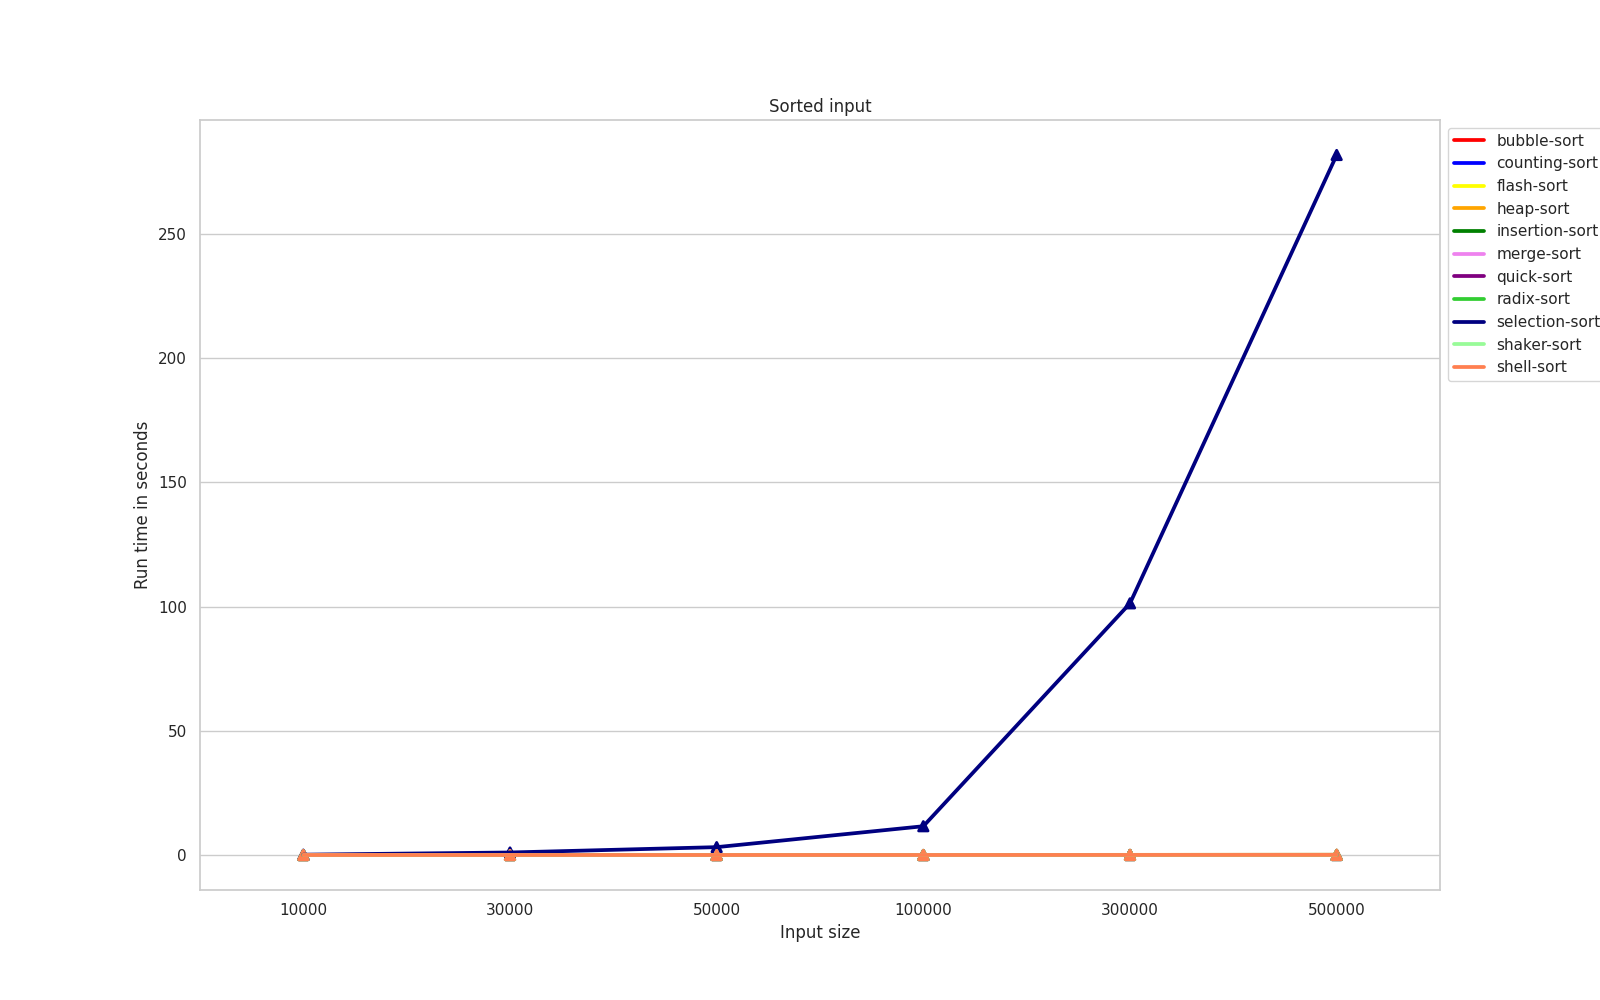
\includegraphics[width = 16cm]{plot/sorted_line.png}
  \centering
  \caption{Visualizing the algorithms' running times on sorted data}
\end{figure}

\begin{figure}[H]
  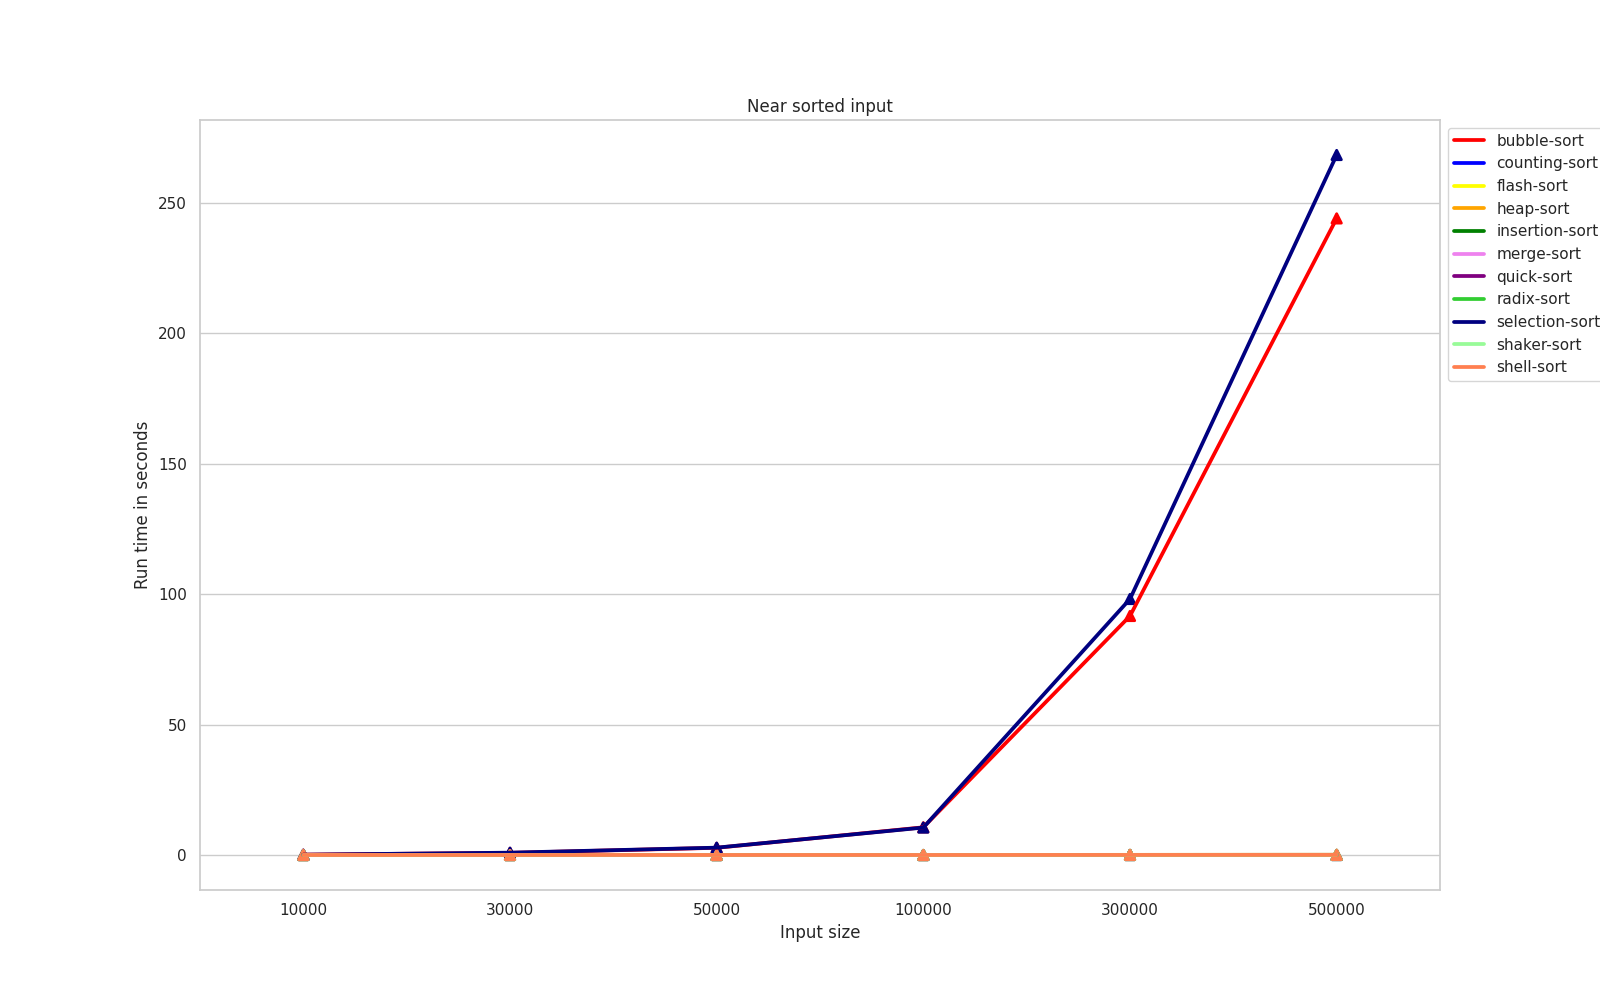
\includegraphics[width = 16cm]{plot/nsorted_line.png}
  \centering
  \caption{Visualizing the algorithms' running times on nearly sorted data}
\end{figure}

\begin{figure}[H]
  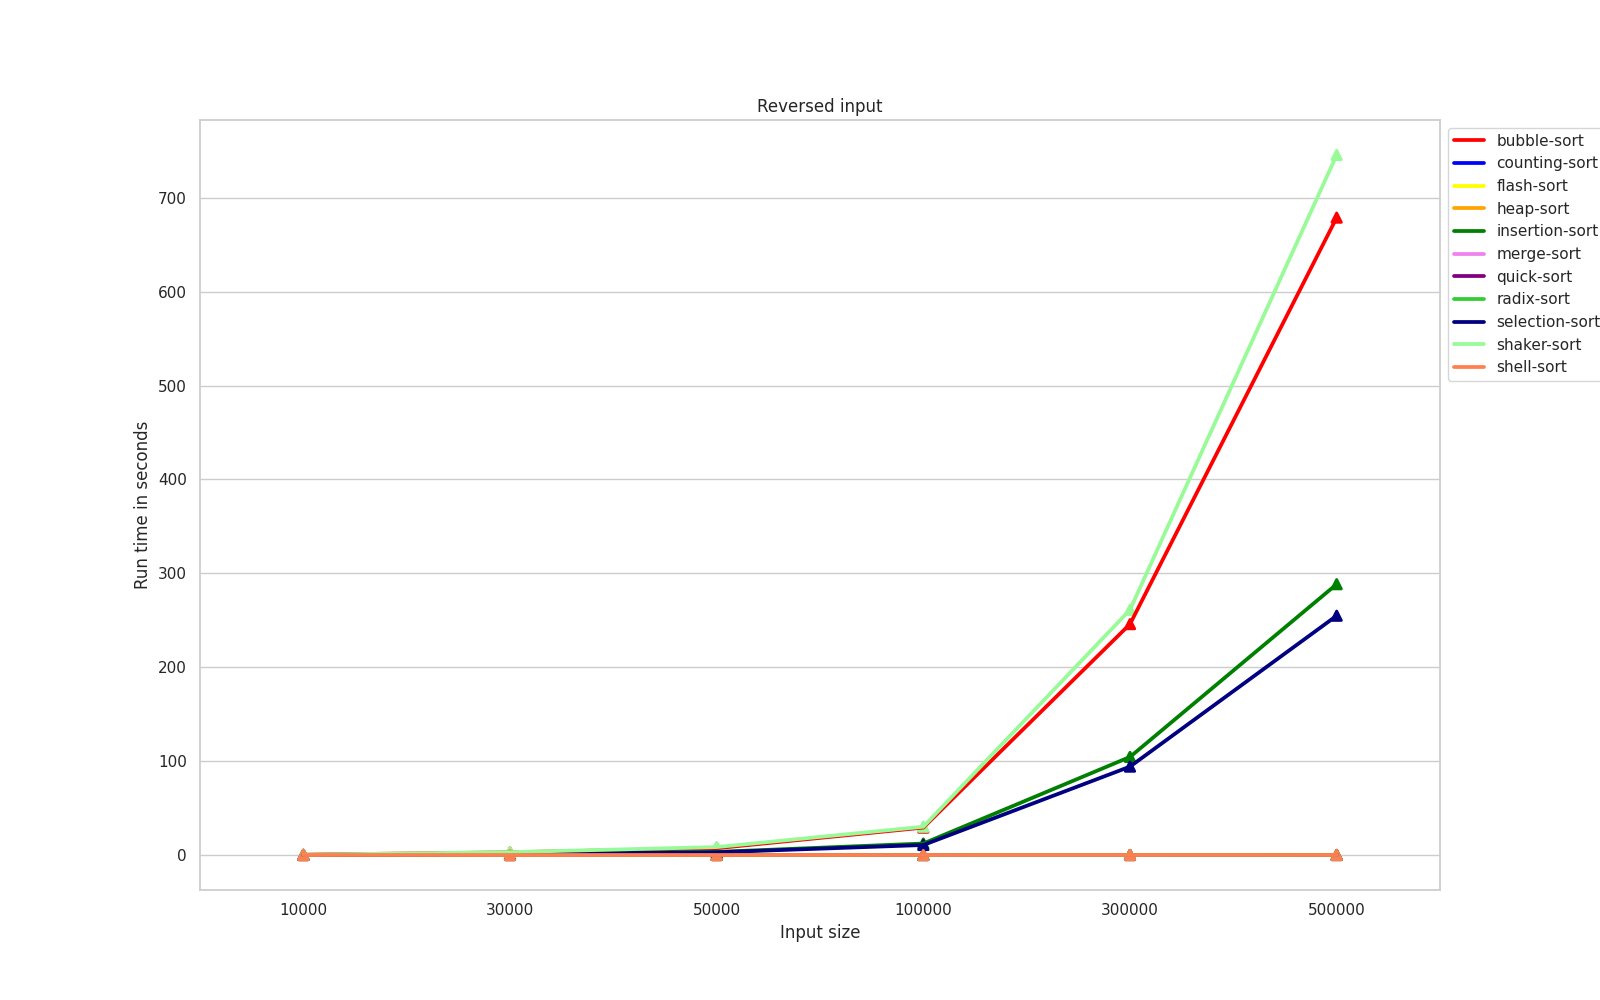
\includegraphics[width = 16cm]{plot/rev_line.png}
  \centering
  \caption{Visualizing the algorithms' running times on reverse sorted data}
\end{figure}

\begin{figure}[H]
  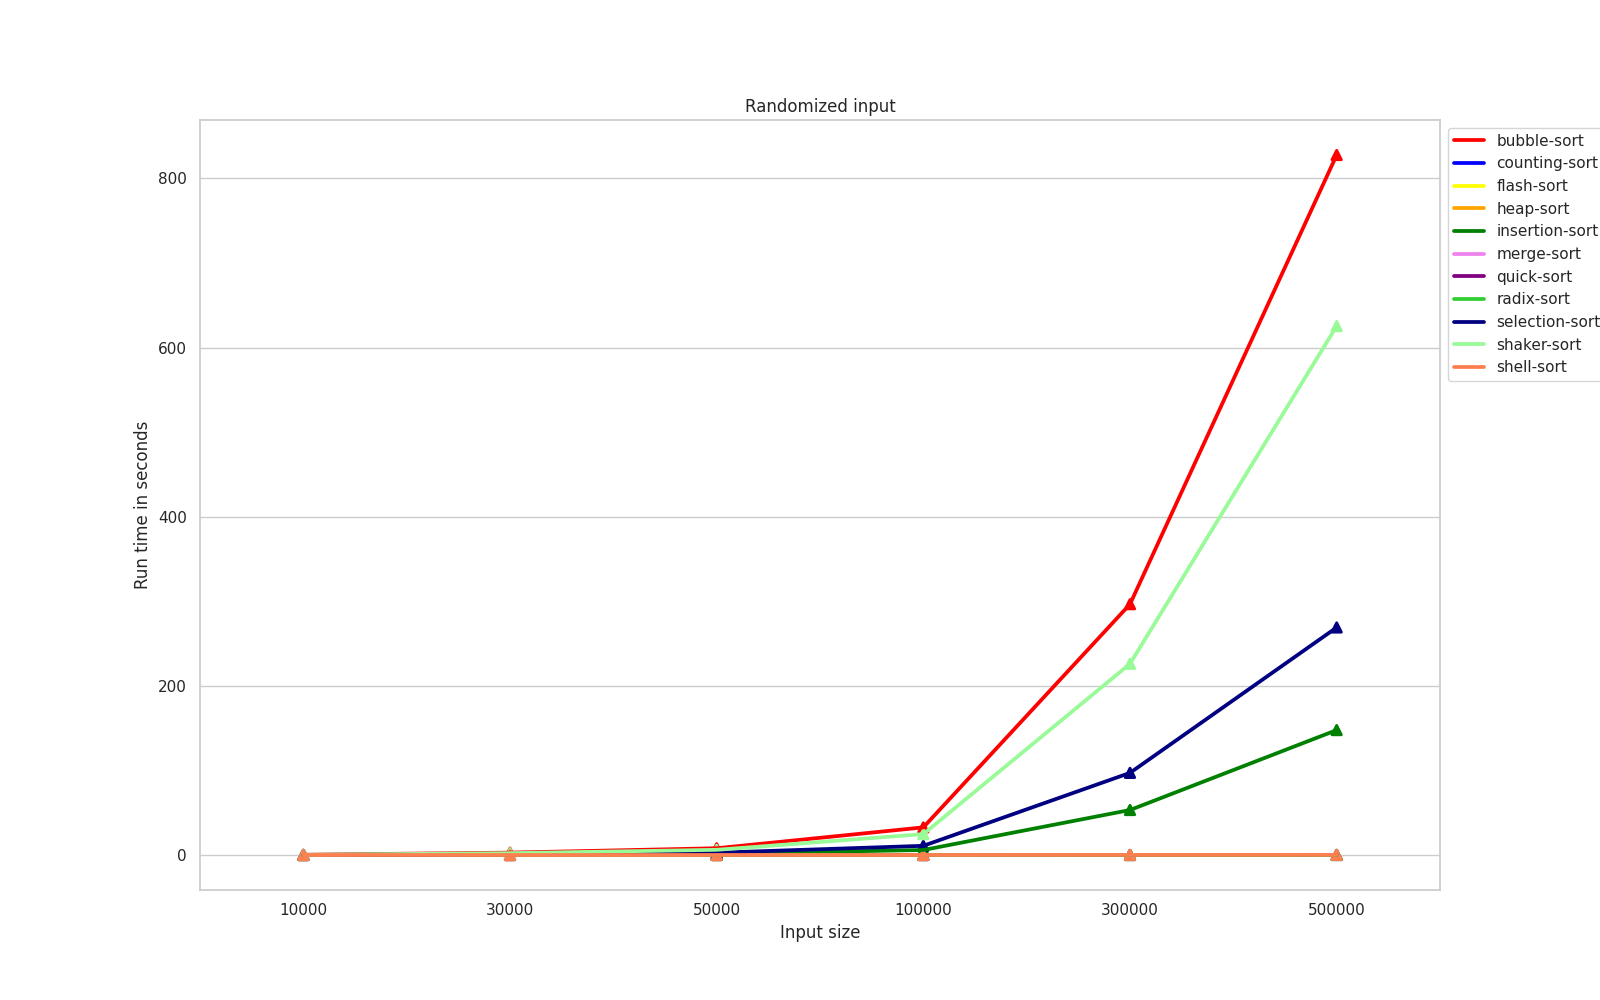
\includegraphics[width = 16cm]{plot/rand_line.png}
  \centering
  \caption{Visualizing the algorithms' running times on randomized data}
\end{figure}

\begin{figure}[H]
  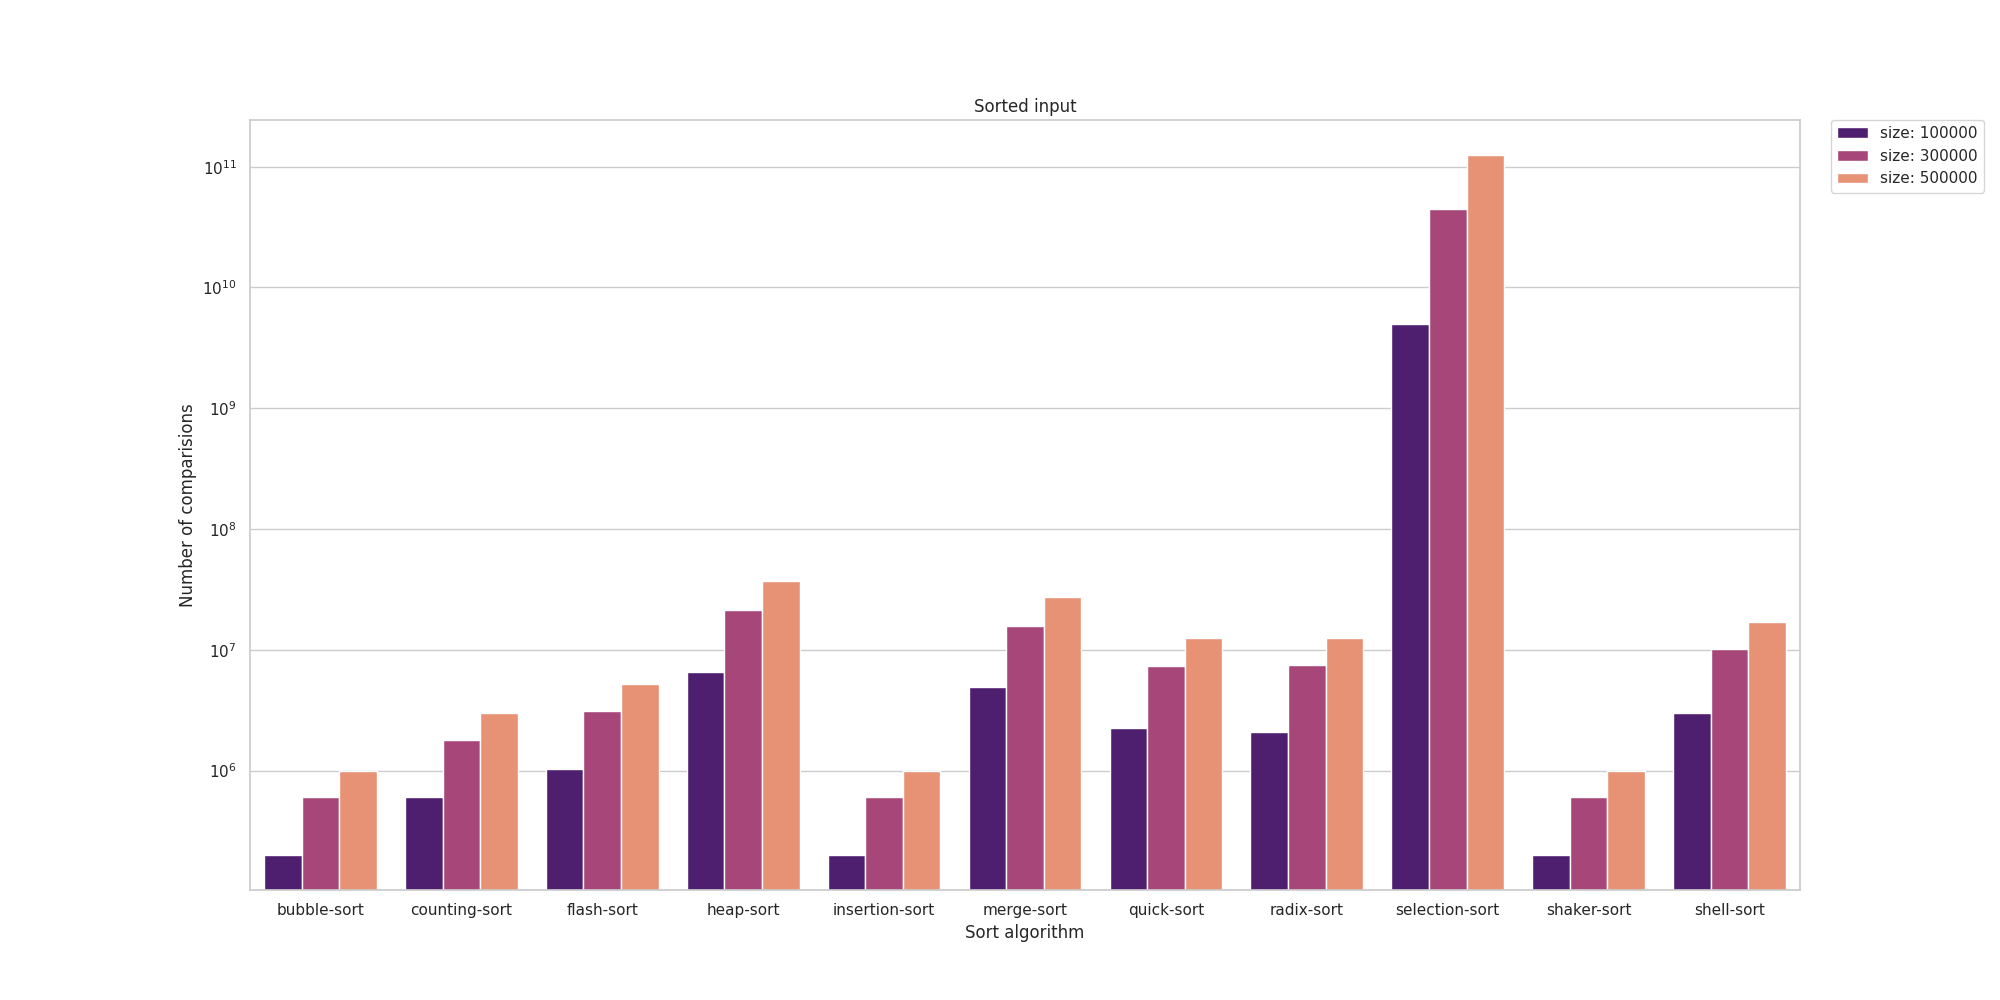
\includegraphics[width = 16cm]{plot/sorted_bar.png}
  \centering
  \caption{Visualizing the algorithms' numbers of comparisons on sorted data}
\end{figure}

\begin{figure}[H]
  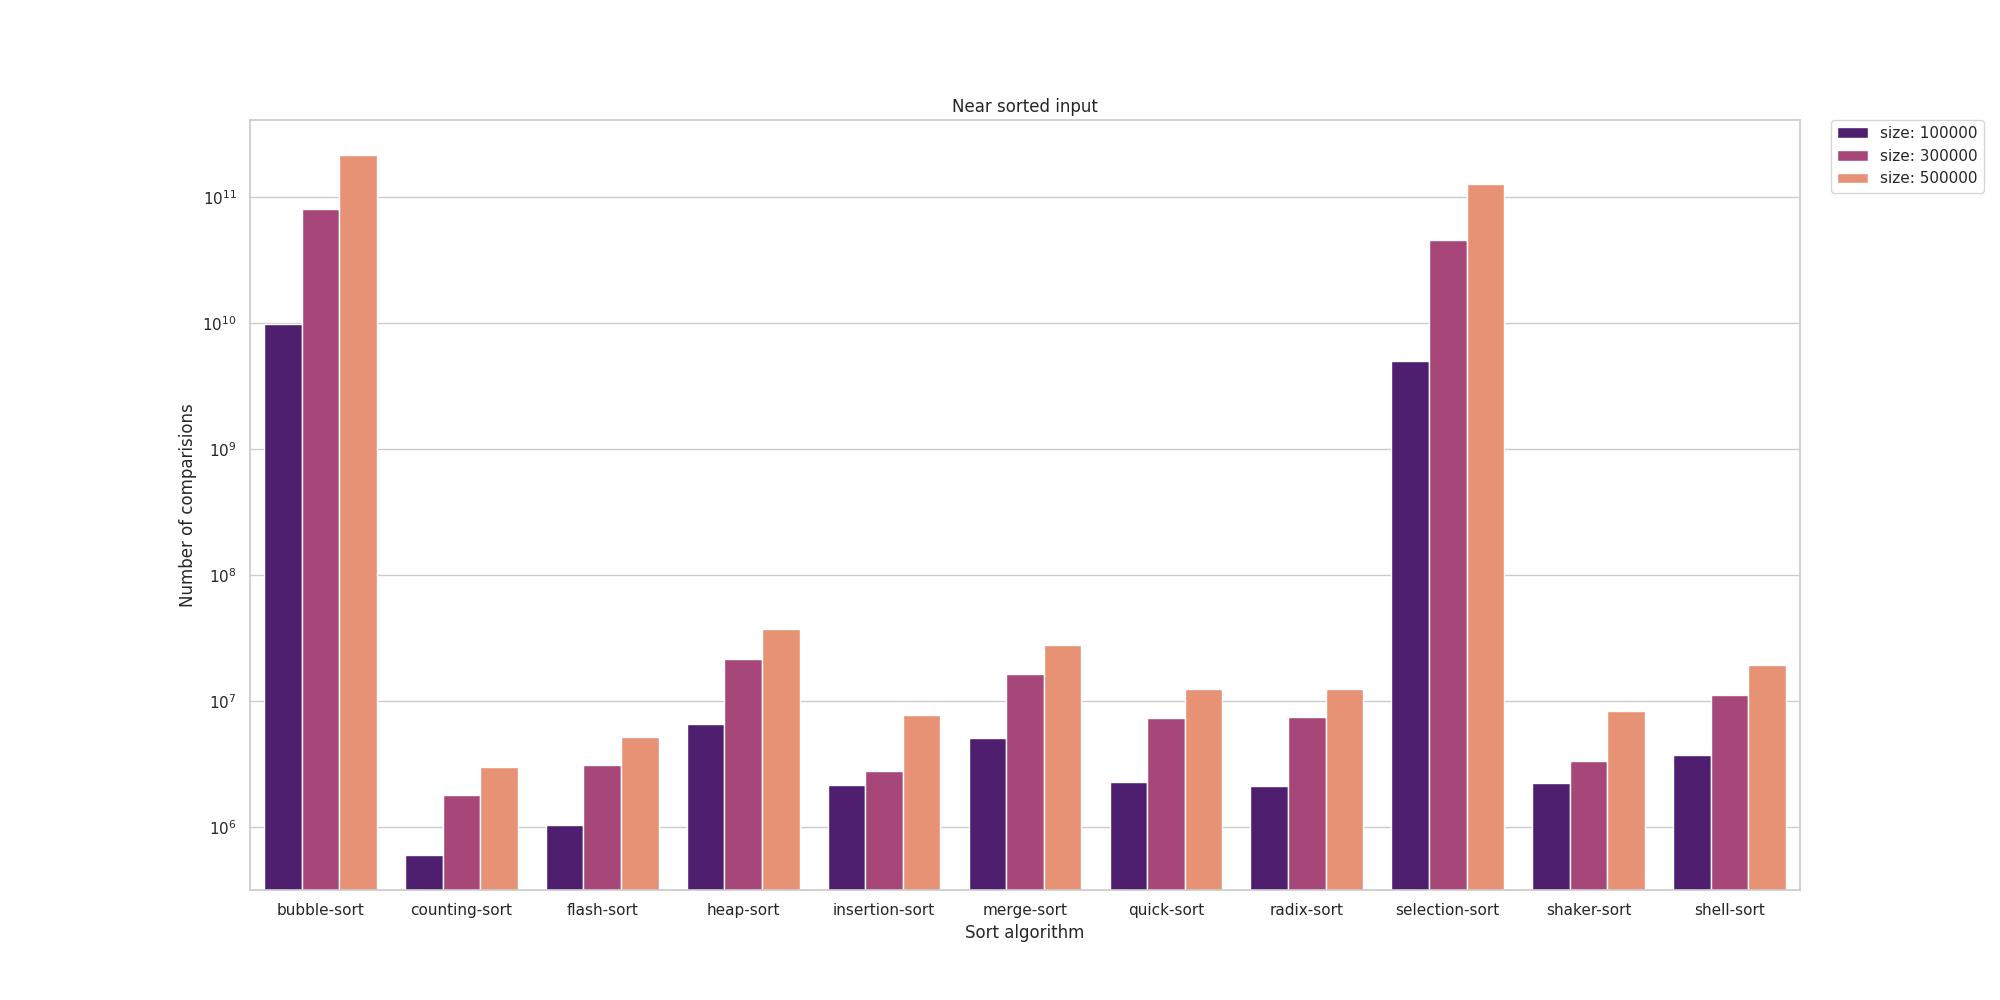
\includegraphics[width = 16cm]{plot/nsorted_bar.png}
  \centering
  \caption{Visualizing the algorithms' numbers of comparisons on nearly sorted data}
\end{figure}

\begin{figure}[H]
  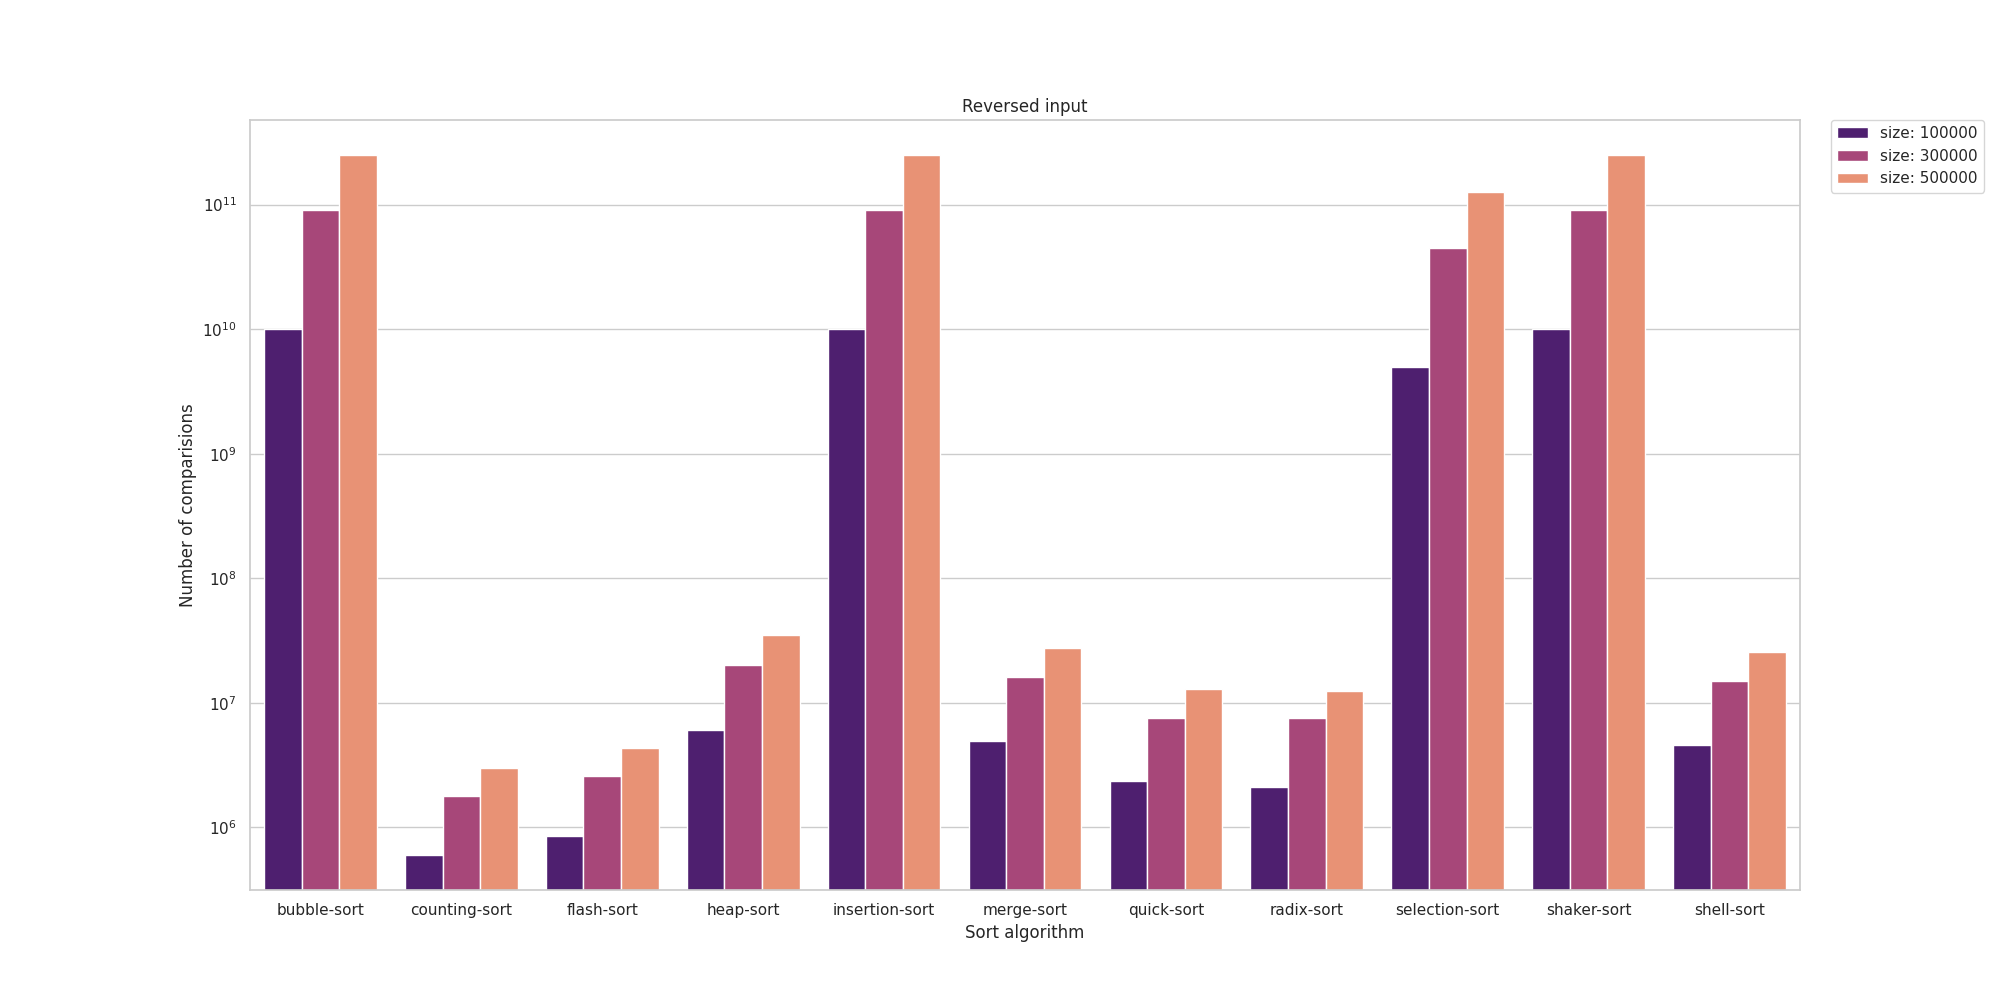
\includegraphics[width = 16cm]{plot/rev_bar.png}
  \centering
  \caption{Visualizing the algorithms' numbers of comparisons on reverse sorted data}
\end{figure}

\begin{figure}[H]
  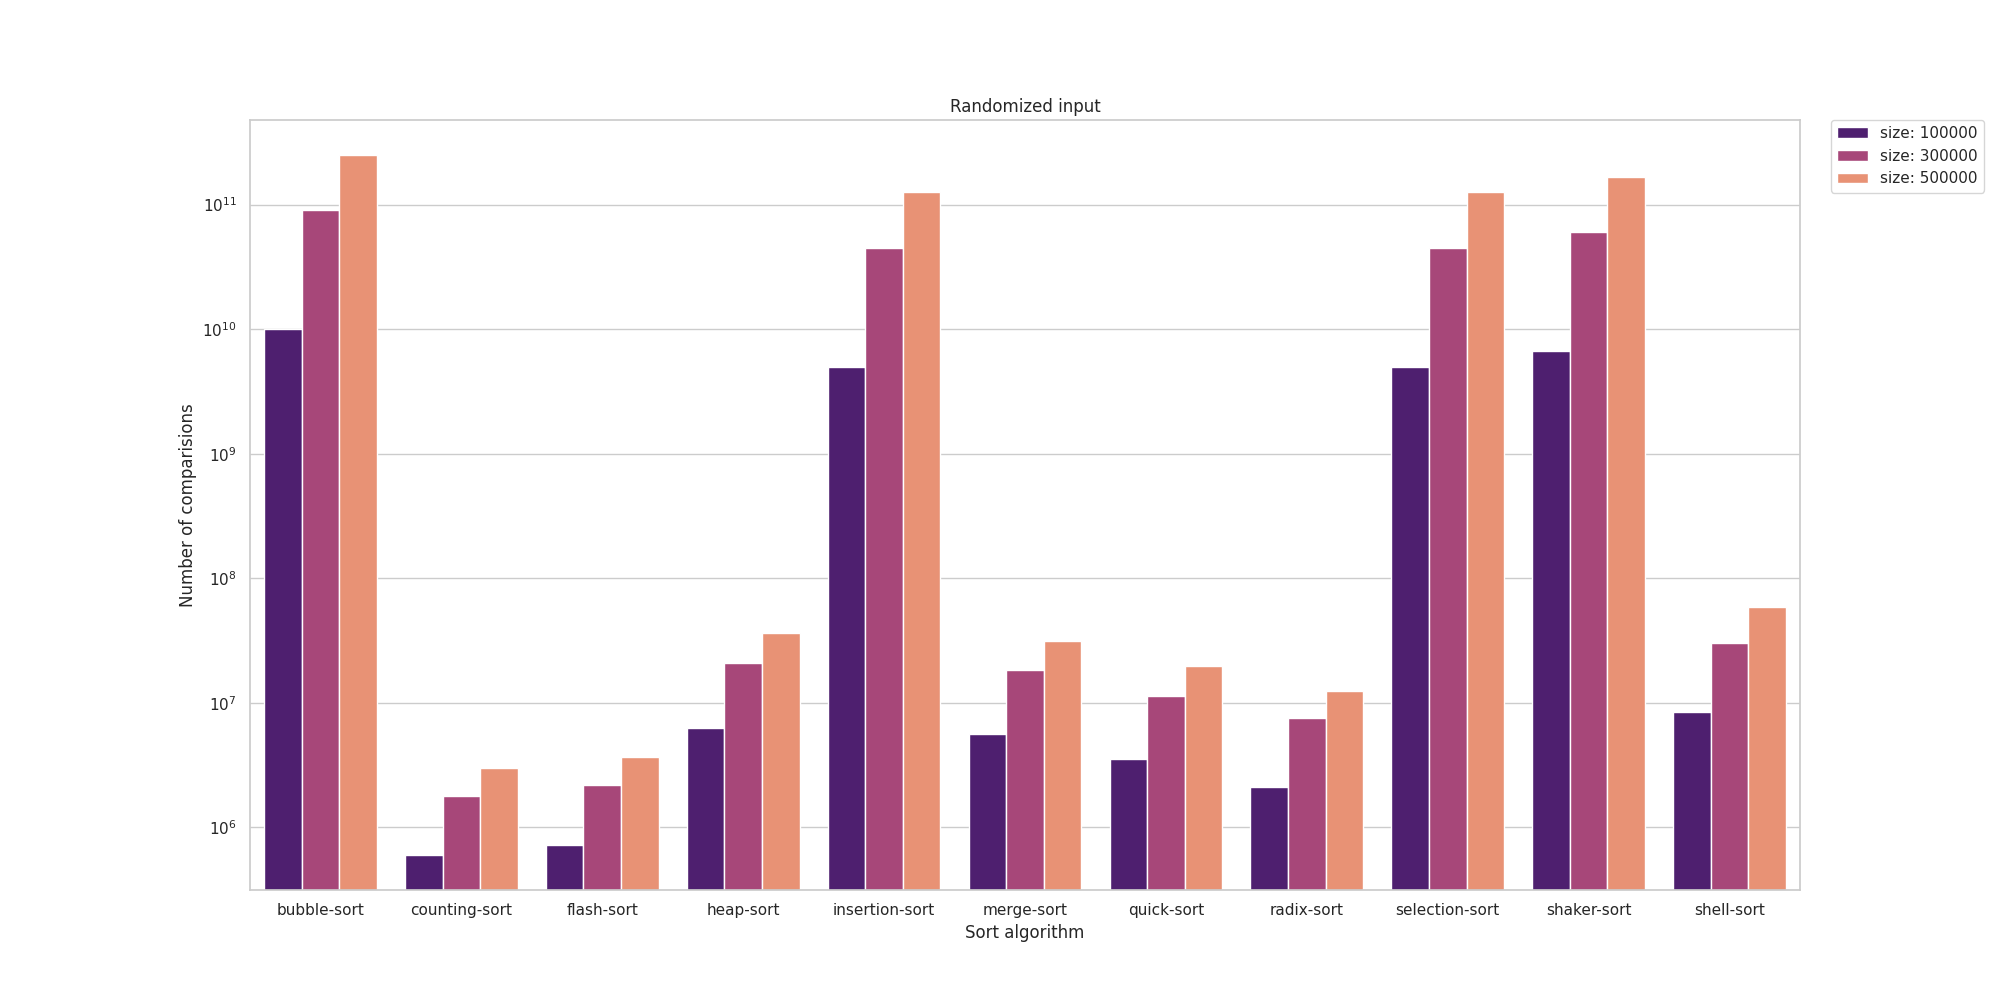
\includegraphics[width = 16cm]{plot/rand_bar.png}
  \centering
  \caption{Visualizing the algorithms' numbers of comparisons on randomized data}
\end{figure}

\section{Project organization}
C++ programming language was used in sorting algorithms' implementation.
Python programming language and open libraries (Pandas, Matplotlib, Seaborn) were used in processing data and graphical visualizing.
\newline
Source code: \url{https://github.com/huynhtuan17ti/Sorting-Overview}

\section{References}
\begin{enumerate}
  \item \url{https://www.geeksforgeeks.org/} (Explanations and source code of several sorting algorithms)\\
  \item \url{https://www.wikipedia.org/} (Scientific explanations of all sorting algorithms)\\
  \item \url{https://www.researchgate.net/publication/315662067_Sorting_Algorithms_-_A_Comparative_Study}\\
  \item \url{https://www.researchgate.net/publication/259911982_Review_on_Sorting_Algorithms_A_Comparative_Study}\\
  \item Introduction to Algorithms (Third edition)\\
\end{enumerate}

\end{document}